\documentclass{report}

\usepackage{polski} % Pozwala na użycie polskiego. Ustawia między innymi fontenc na T1
\usepackage[utf8]{inputenc} % Informuje o kodowaniu

\usepackage{xcolor}% http://ctan.org/pkg/xcolor
\usepackage{hyperref}% http://ctan.org/pkg/hyperref

\definecolor{LinkColor}{HTML}{1d5cc1}

\usepackage{tabto}

\usepackage{graphicx} % Pakiet do obrazów
\graphicspath{ {./Obrazy/} } % Folder, z którego będą brane obrazy

% Nie twórz nowych stron
\usepackage{etoolbox}
\makeatletter
% \patchcmd{\chapter}{\if@openright\cleardoublepage\else\clearpage\fi}{}{}{}
\makeatother

\title{Specyfikacja funkcjonalna -- Wireworld}
\author{Krzysztof Dąbrowski i Jakub Bogusz}
\date{\today}

\begin{document}
\maketitle{}

\tableofcontents{}

\chapter{Cel projektu}
Celem projektu jest implementacja automatu komórkowego Wire World w języku Java z interfejsem graficznym zaimplementowanym przy pomocy biblioteki JavaFX. Gotowy program ma pozwalać użytkownikowi przeprowadzać symulacje zgodne z określonymi zasadami. Parametrami generacji użytkownik będzie mógł sterować ręcznie z wbudowanego menu opisanego niżej [TU DAĆ LINK DO SEKCJI Z GRAFIKĄ I OPISEM CZĘŚCI].
%TODO: Link do GUI
Interfejs będzie wyświetlał na bierząco podgląd kolejnych generacji. Użytkownik będzie miał możliwość wstrzymania symulacji oraz zmianę stanu planszy przy pomocy narzędzi edycji.

Ponadto będzie istnieć również możliwość przełączenia trybu symulacji z Wire World na automat komórkowy Game of life.

\chapter{Opis ogólny problemu}

\section{Wstęp}
Projektu skupia się na realizacji 3 głównych aspektów problemu. Są to odpowiednio automaty komórkowe ,,Game of Life'' i ,,Wireworld'' oraz wizualna prezentacja działania tych automatów. 

\section{Wire World}

Wire World jest automatem komórkowym wymyślonym przez Briana Silvermana w roku 1987.  Jest często używany do symulacji elementów elektronicznych operujących na wartościach bitowych. Pomimo prostoty reguł, jakie nim rządzą, za pomocą Wireworld można nawet stworzyć działający komputer.

\subsection{Symulacja}
\begin{minipage}{\textwidth} %Akapit ma być na jednej stronie
    \paragraph{Stany}  Komórka może znajdować się w jednym z czterech stanów:
    \begin{itemize}
    \item pusta,
    \item głowa elektronu,
    \item ogon elektronu,
    \item przewodnik.
    \end{itemize}
\end{minipage}

\paragraph{Pokolenie} to zbiór stanów wszystkich komórek w danej chwili. Gdy stan pokolenia jest ustalony, możliwe jest utworzenie nowego (potomnego) pokolenia komórek, powstających według poniższych zasad.

\paragraph{Reguły} Następne pokolenie generowane jest zgodnie z regułami:
\begin{itemize}
\item Jeżeli komórka jest pusta, to pozostaje pusta niezależnie od jej otoczenia,
\item Jeżeli komórka jest głową elektronu, to zmieni się w ogon elektronu,
\item Jeżeli komórka jest ogonem elektronu, to zmieni się w przewodnik,
\item Jeżeli komórka jest przewodnikiem i sąsiaduję z jedną lub dwoma komórkami będącymi głowami elektronu, to zmieni się w przewodnik.
\end{itemize}

\subsection{Struktury}
Symulacja przeprowadzona zgodnie z powyższymi regułami może prowadzić do powstania ciekawych obiektów zwanych strukturami. 
\begin{figure}[h]
\centering
\setlength{\fboxsep}{0pt} %Odstęp 0
\setlength{\fboxrule}{1pt} %Grubość ramki 1p
\fbox{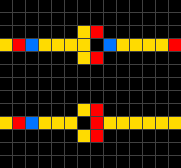
\includegraphics[width=8cm]{Obrazy/struktury_w.png}}
\caption{Przykłady struktur - dioda przewodząca i nieprzewodząca}
\end{figure}


\section{Game of life}

Game of life jest automatem komórkowym wymyślonym przez brytyjskiego matematyka John Horton Conway
w 1970 roku. Polega na symulacji kolejnych pokoleń życia komórek według następujących zasad.

\subsection{Symulacja}

\paragraph{Stany}  Komórka może znajdować się w jednym z dwóch stanów:
\begin{itemize}
\item żywa,
\item martwa.
\end{itemize}

\paragraph{Pokolenie} to stan wszystkich komórek w danej chwili. Gdy stan pokolenia jest ustalony, możliwe jest utworzenie nowego (potomnego) pokolenia komórek, powstających według poniższych zasad.

\paragraph{Reguły} Następne pokolenie generowane jest zgodnie z regułami:
\begin{itemize}
\item Jeżeli komórka była martwa i miała dokładnie 3 żywych sąsiadów, w następnym pokoleniu staje się żywa,
\item Jeżeli komórka była żywa to pozostaje żywa jeśli miała dwóch lub trzech żywych sąsiadów. W przeciwnym razie staje się martwa.
\end{itemize}

\subsection{Struktury}
Symulacja przeprowadzona zgodnie z powyższymi regułami może prowadzić do powstania ciekawych obiektów zwanych strukturami. 

\begin{figure}[h]
\centering
\setlength{\fboxsep}{0pt} %Odstęp 0
\setlength{\fboxrule}{1pt} %Grubość ramki 1p
\fbox{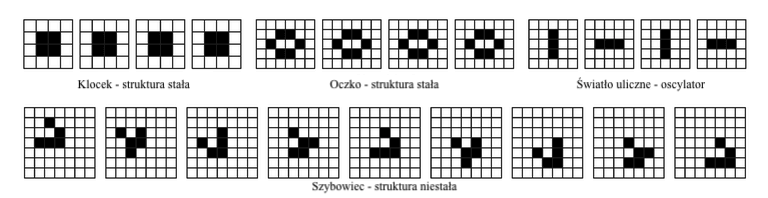
\includegraphics[width=13cm]{Obrazy/struktury.png}}
\caption{Przykłady struktur}
\end{figure}

Reguły symulacji umożliwiają również tworzenie dużo bardziej skomplikowanych struktur (jak na przykład maszyna Turinga -- https://youtu.be/My8AsV7bA94).

\section{Interfejs użytkownika}
\label{sec:opis-interfejs}
Ważnym aspektem programu jest sposób interakcji z użytkownikiem.
Realizowana aplikacja będzie obsługiwana poprzez graficzny interfejs użytkownika.

Interfejs pozwoli na poniższe funkcjonalności:
\begin{itemize}
    \item Bieżący podgląd stanu symulacji
    \item Możliwość dostosowania prędkości symulacji
    \item Zapis aktualnego pokolenia do pliku
    \item Wyczytanie pokolenia z pliku
    \item Edycje poszczególnych komórek w trakcie symulacji
    \item Wstawianie figur wybranch z przybornika
\end{itemize}

\chapter{Działanie programu}

\section{Opis komunikacja z użytkownikiem}
Po programu zostanie wyświetlony graficzny interfejs, który pozwoli użytkownikowi sterować parametrami w dowolny sposób, zgodny z regułami symulacji. W razie wystąpienia błędów program będzie informować użytkownika wyświetlając nowe okno zawierające opis błędu.

W ramach interfejsu użytkownik będzie mógł wykonywać czynności opisane w punkcie \ref{sec:opis-interfejs} oraz przełączać między automatami Game of Life i Wireworld.

\section{Wygląd interfejsu użytkownika}
Poniżej przedstawiony jest szkic interfejsu użytkownika w różnych stanach.

\subsection{Po włączeniu programu}
Większość kontrolek jest \textbf{wyłączonych} do momentu wczytania planszy z pliku lub wygenerowania losowej. Program domyślnie wyświetla okno symulacji automatu Wireworld.

\subsection{W trakcie symulacji}
Można zmienić tempo symulacji oraz wstrzymać generację następnych pokoleń, co umożliwi edycję aktualnego pokolenia.

\subsection{Symulacja wstrzymana}
Możliwe jest edytowanie komórek przy pomocy narzędzie i wstawianie figur.

\subsection{Tryb automatu Game of Live}

%\begin{figure}[h]
%\centering
%\setlength{\fboxsep}{0pt} %Odstęp 0
%\setlength{\fboxrule}{1pt} %Grubość ramki 1p
%\fbox{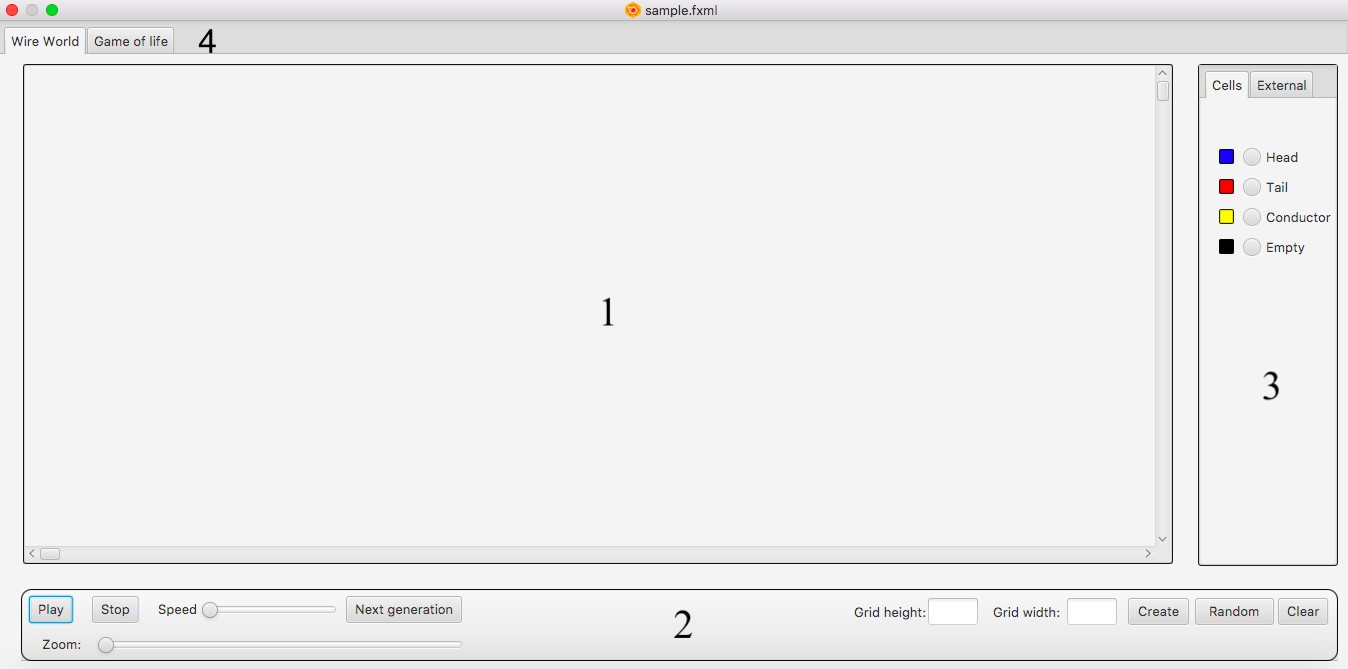
\includegraphics[width=13cm]{Obrazy/gui.png}}
%\caption{Przykłady struktur}
%\end{figure}


\section{Plik wejściowy}  \label{format}
Plik wejściowy pozwala na wczytanie stanu planszy. Dzięki temu użytkownik ma kontrolę nad początkiem symulacji, oraz może kontynuować symulacje z zapisanego wcześniej etapu.

\subsection{Przykład}
5 3 \tab -- rozmiar (x y) \\
1 0 0 1 1 \tab -- Wartości poszczególnych komórek \\
0 1 1 0 1 \tab -- 1 - żywa \\
0 0 0 1 1 \tab -- 0 - martwa \\

\subsection{Format pliku}
\subsubsection*{Kodowanie}
Ponieważ plik powinien zawierać tylko liczby arabskie i odstępy możliwe jest dowolne kodowanie kompatybilne z ASCII. \\
\paragraph{Sugerowane kodowania to:}
ASCII, UTF-8, ISO 8859, Windows-1250

\subsubsection*{Opis formatu}
Plik w pierwszej linii powinien zawierać 2 liczby. Pierwsza z nich oznacza rozmiar planszy w poziomie, druga w pionie. \\
Następnie plik powinien zawierać tyle linii jaki został podany rozmiar w pionie. W każdej z tych linii powinno być tyle 0 lub 1 ile wynosi rozmiar w poziomie. \\
Zero oznacz komórkę martwą, a jeden komórkę żywą.

\chapter{Wyniki działania programu}
Wyniki działania programu będą zależeć od preferencji użytkownika -  od podanych \hyperref[argumenty]{\textcolor{LinkColor}{argumentów}}. 
\begin{itemize}
\item wyświetlić wybraną ilość pokoleń w konsoli,
\item wygenerować plik lub pliki .png z reprezentacjami graficznymi kolejnych pokoleń,
\item wygenerować plik .gif przedstawiający życie cywilizacji,
\item wygenerować plik lub pliki .txt reprezentujący konkretny stan cywilizacji, mogący służyć za plik wejściowy.
\end{itemize}

\chapter{Sytuacje wyjątkowe}
Czasem działanie programu może ulec zmianie na skutek nieprawidłowych danych wejściowych, niestandardowych ustawień wprowadzonych przez użytkownik lub z przyczyn losowych. Ten rozdział opisuje jak program zachowa się w takiej sytuacji, oraz co może ją wywołać.

\section{Zmiana domyślnego zachowania}
\paragraph{Zbyt szeroka plansza}
W przypadku gdy użytkownik włączy wyświetlanie kolejnych stanów w konsoli ale rozmiar planszy będzie zbyt szeroki by możliwe było jej wyświetlenie bez zawijania wierszy program wyświetli komunikat o niemożliwości wyświetlenia planszy w konsoli. Kolejne pokolenia nie będą wyświetlanie oknie wiersza poleceń ale generacja plików wynikowych nie ulegnie zmianie. \\
Treść komunikatu: ,,Wybrana szerokość planszy jest zbyt duża by możliwe było wyświetlenie kolejnych pokoleń w oknie konsoli.''

\section{Błędy}
Opis błędów, które mogą wystąpić w trakcie działania programu.

\subsection{Błędy pliku wejściowego}

\paragraph{Podany plik nie istnieje}
Jeśli ścieżka podana przez użytkownika jest błędna program wyświetli komunikat o braku możliwości otwarcia wskazanego pliku i zakończy pracę. \\
Treść komunikatu: ,,Nie udało się otworzyć wskazanego pliku.''

\paragraph{Pusty plik}
W przypadku gdy plik wskazany przez użytkownika będzie pusty program powiadomi o tym i zakończy pracę. \\
Treść komunikatu: ,,Wskazany plik wejściowy jest pusty.''

\paragraph{Rozmiar planszy nie będący liczbą}
Jeśli w pierwszej lini pliku znajdować się będą wartości inne niż liczby program nie będzie w stanie wczytać rozmiaru planszy. W takiej sytuacji wyświetli odpowiedni komunikat i zakończy pracę. \\
 Treść komunikatu: ,,Nie udało się wczytać rozmiaru planszy.''
 
 \paragraph{Niedodatni rozmiar planszy}
 Jeśli jeden z wymiarów planszy nie będzie dodatnią liczbą całkowitą program zasygnalizuje błąd i zakończy pracę. \\
 Przykładowy komunikat: ,,Szerokość musi być większa od 0. Podana szerokość to -5.''
 
 \paragraph{Brak nowej linii po rozmiarze planszy}
 W przypadku gdy po wysokości planszy w pliku będzie inny znak niż przejście do nowej lini program zasygnalizuje błąd i zakończy pracę. \\
 Treść komunikatu: ,,Spodziewany koniec lini po wymiarze planszy.''
 
 \paragraph{Błąd przy wczytywaniu stanu komórki}
 Jeśli nie uda się wczytać stanu komórki, na przykład ponieważ w pliku jest za mało linii lub jedna z linii jest zbyt krótka, program wypisze, w którym miejscu pliku wystąpił błąd i zakończy pracę. \\
 Przykładowy komunikat: ,,Wystąpił błąd przy próbie przeczytania znaku w lini: 3 kolumnie: 8.''
 
 \paragraph{Nieprawidłowy znak w pliku}
 Jeśli podczas czytania pliku program napotka nieprawidłowy znak wypisze na jakiej pozycji w pliku napotkany został nieprawidłowy znak, jaki to znak, oraz czego spodziewał się program. \\
 Przykładowy komunikat: ,,Niewspierany znak napotkany w lini: 2 kolumnie: 1. Spodziewana wartość: 0 lub 1. Napotkana wartość: T''

\subsection{Błędy losowe}
\paragraph{Brak pamięci operacyjnej}
Gdyby w systemie zabrakło pamięci program nie będzie w stanie funkcjonować poprawnie. Program wyświetli komunikat o błędzie i przerwie pracę. \\
Treść komunikatu: ,,Program nie uzyskał pamięci od systemu operacyjnego. Spróbuj uruchomić program ponownie za pewien czas.''

\end{document}
